\documentclass[sigconf,nonacm]{acmart}
\settopmatter{printacmref=false,printfolios=true}
\setcopyright{none}
\renewcommand\footnotetextcopyrightpermission[1]{}
\usepackage{amsmath,tabularx,array,enumitem,balance,tikz}
\usetikzlibrary{arrows.meta,positioning,shapes.geometric}
\definecolor{CourseBlue}{HTML}{315EFB}
\definecolor{CourseTeal}{HTML}{14877D}
\definecolor{CourseInk}{HTML}{18324A}
\hypersetup{colorlinks=true,linkcolor=CourseBlue,citecolor=CourseTeal,urlcolor=CourseTeal}
\newcolumntype{Y}{>{\raggedright\arraybackslash}X}
\setlist{leftmargin=*,topsep=3pt,itemsep=2pt}
\newcommand{\CourseNumber}{COMSCI/ECON 206}
\newcommand{\CourseName}{Computational Microeconomics}
\newcommand{\CourseSession}{Autumn 2026 Session 1}
\newcommand{\Instructor}{Professor Luyao Zhang}
\newcommand{\TeamCode}{[FPXX]}
\newcommand{\SymposiumSession}{[A/B/C/D]}
\newcommand{\GitHubLink}{[Your team GitHub repository and exact commit/release]}
\newcommand{\NotebookLink}{[Your runnable notebook URL]}
\newcommand{\HuggingFaceLink}{[Your behavioral-science Hugging Face repository or Space]}
\newcommand{\PosterLink}{[Your editable A0 poster filename or stable URL]}
\newcommand{\coursemeta}{\noindent\textbf{Submission to:} \CourseNumber{} --- \CourseName.\\
\textbf{Course session:} \CourseSession. \textbf{Team:} \TeamCode. \textbf{Symposium:} \SymposiumSession.\\
\textbf{Course instructor:} \Instructor. \textbf{Assignment:} PS2 collaborative research proposal.\par\smallskip}
\title{[A Specific, Researchable Collaborative Proposal Title]}
\author{[Member 1 Full Name]}
\affiliation{\institution{Duke Kunshan University}\city{Kunshan}\country{China}}
\email{[Member 1 university email]}
\author{[Member 2 Full Name]}
\affiliation{\institution{Duke Kunshan University}\city{Kunshan}\country{China}}
\email{[Member 2 university email]}
\author{[Member 3 Full Name]}
\affiliation{\institution{Duke Kunshan University}\city{Kunshan}\country{China}}
\email{[Member 3 university email]}
\renewcommand{\shortauthors}{Team \TeamCode}

% The instructor is course metadata, not a paper author.
% The annotated driver keeps this same paper layout and adds a printable side rail.
\newif\ifTeachingAnnotations
\TeachingAnnotationstrue
% Visible, printable teaching notes. The original ACM text area is unchanged.
% Use main.tex for the clean submission and annotated.tex for guidance.
\ifTeachingAnnotations
\usepackage{eso-pic,tikz}
\usepackage[most]{tcolorbox}
\definecolor{AnnReplace}{HTML}{245BB4}
\definecolor{AnnConnect}{HTML}{08756C}
\definecolor{AnnDevelop}{HTML}{79469C}
\definecolor{AnnInk}{HTML}{21324A}
\definecolor{AnnRail}{HTML}{F4F6FA}
\definecolor{AnnLine}{HTML}{D4DCE7}
\newsavebox{\AnnRailBox}
\newcommand{\AnnNote}[4]{%
  \begin{tcolorbox}[enhanced,sharp corners,boxrule=0pt,frame hidden,
    colback=#2!5!white,borderline west={2pt}{0pt}{#2},
    left=7pt,right=7pt,top=5pt,bottom=5pt,before skip=6pt,after skip=0pt]
    \sffamily\fontsize{9.4}{11.8}\selectfont\color{AnnInk}\raggedright
    {\color{#2}\bfseries #1\quad #3}\par\vspace{2pt}#4
  \end{tcolorbox}}
\newcommand{\AnnPin}[4]{%
  \node[rounded corners=2bp,fill=#2,text=white,inner xsep=4bp,
    inner ysep=2.5bp,font=\sffamily\bfseries\fontsize{8}{9}\selectfont]
    at (#3,#4) {#1};}
\newcommand{\AnnPageTitle}{%
  \ifcase\value{page}\or
    Keep the PS1 structure\or
    Integrate evidence and impact\or
    Preserve the appendix sequence\or
    Update the same cumulative map\or
    Add only the PS2 extension record\else
    Continue the documented draft\fi}
\newcommand{\AnnPageNotes}{%
  \ifcase\value{page}\or\AnnNote{R1}{AnnReplace}{Replace team identity, not course identity}{%
Replace the title, team code, symposium session, member names, and emails. Keep the course, term, and \textbf{Course instructor: Professor Luyao Zhang}. The instructor is metadata, not a paper author.}

\AnnNote{R2}{AnnReplace}{Adapt the LaTeX-native teaser}{%
Edit \texttt{figures/ps2\_teaser.tex}. Keep the three evidence panels and synthesis logic, but replace their content with your actors, model, computation, behavioral test, A0-poster claim, and real-world case.}

\AnnNote{C1}{AnnConnect}{Keep the familiar five-section spine}{%
Section 1 asks the connected questions. Sections 2--4 answer the economics, computation, and behavior questions. Section 5 states the integrated contribution and practical impact. Carry the same claims into Appendix E.}

\AnnNote{D1}{AnnDevelop}{Choose the correct solution concept}{%
Define players, strategies, timing, information, beliefs, and payoffs before naming an equilibrium. Translate the same problem through game theory, social choice, and mechanism design; show what changes.}
\or
    \AnnNote{C2}{AnnConnect}{Make behavioral evidence consequential}{%
Use self-reflection and peer play to probe an assumption. State the competing explanation and the observation that would make the team retain, qualify, or revise the model, algorithm, or interface.}

\AnnNote{D2}{AnnDevelop}{Connect the real-world case to evidence}{%
Identify stakeholders, feasible benefit, risk, missing evidence, and correction route. Compare the standards of academia, industry, and public institutions without claiming impact that has not been measured.}

\AnnNote{R3}{AnnReplace}{Use the confirmed dates}{%
Review-ready: September 27 at 11:00 P.M. Symposium, peer evaluation, and practical-impact discussion: September 28. Final revision: September 30 at 11:00 P.M., before the October 1--2 holiday.}
\or\AnnNote{R4}{AnnReplace}{Credit people and work accurately}{%
Keep Professor Luyao Zhang as course instructor. Acknowledge peers, discussants, partners, data, software, adapted materials, and AI assistance only when used. Give each author an inspectable intellectual decision and output.}

\AnnNote{D3}{AnnDevelop}{Appendices A and B remain familiar}{%
Appendix A holds technical details, reproducibility, and AI disclosure. Appendix B retains the PS1 change record: earlier claim, dated evidence or feedback, revision, and intellectual consequence.}

\AnnNote{C3}{AnnConnect}{Appendices C and D preserve continuity}{%
Appendix C records open-source inspirations and the three-lens stress test. Appendix D preserves review, response, rerun, and revision. Do not replace missing feedback with invented evidence.}
\or
    \AnnNote{R5}{AnnReplace}{Complete the same eight rows}{%
Appendix E deliberately retains the PS1 structured abstract. Replace each prompt, save the prior version, and use complete, specific sentences.}

\AnnNote{C4}{AnnConnect}{Rows 1--4 must match Sections 1--3}{%
Use the same gap, application, connected questions, actors, incentives, timing, information, baseline, and evidence status. A reader should not encounter a different model in the table.}

\AnnNote{D4}{AnnDevelop}{Rows 5--8 close the evidence loop}{%
Separate actual and expected results. Explain the integrated intellectual merit and bounded practical impact. Record the dated feedback, revision location, verification, and consequence.}
\or\AnnNote{D5}{AnnDevelop}{Record the auction, not only the outcome}{%
State values or signals, prediction, bid, allocation, payment, stopping rule, utility, revenue, efficiency, behavioral observation, and revision for each treatment.}

\AnnNote{C5}{AnnConnect}{Check parity across three artifacts}{%
GitHub, Hugging Face, and the A0 poster must describe the same question, model, evidence status, result, and limits. The labels describe evidence perspectives, not fixed team roles.}

\AnnNote{D6}{AnnDevelop}{Use the symposium to revise}{%
Retain the September 28 poster and reviews. Record Keep, Revise, or Investigate decisions, rerun the affected check, and identify the exact September 30 change.}
\else
    \AnnNote{D}{AnnDevelop}{Return to the clean driver}{Use \texttt{main.tex} for submission. Recheck the two-page main limit and preserve supporting evidence in the appendices.}
  \fi}
\newcommand{\AnnPagePins}{%
  \ifcase\value{page}\or
    \AnnPin{R1}{AnnReplace}{31}{88}
    \AnnPin{R2}{AnnReplace}{31}{370}
    \AnnPin{C1}{AnnConnect}{31}{510}
    \AnnPin{D1}{AnnDevelop}{581}{400}
  \or
    \AnnPin{C2}{AnnConnect}{31}{94}
    \AnnPin{D2}{AnnDevelop}{31}{240}
    \AnnPin{R3}{AnnReplace}{581}{340}
  \or
    \AnnPin{R4}{AnnReplace}{31}{105}
    \AnnPin{D3}{AnnDevelop}{31}{390}
    \AnnPin{C3}{AnnConnect}{581}{240}
  \or
    \AnnPin{R5}{AnnReplace}{31}{92}
    \AnnPin{C4}{AnnConnect}{31}{260}
    \AnnPin{D4}{AnnDevelop}{31}{420}
  \or
    \AnnPin{D5}{AnnDevelop}{31}{92}
    \AnnPin{C5}{AnnConnect}{31}{310}
    \AnnPin{D6}{AnnDevelop}{581}{260}
  \fi}
\AddToHook{shipout/before}{\global\pdfpagewidth=912bp\relax}
\AddToShipoutPictureBG{\AtPageUpperLeft{%
  \begin{tikzpicture}[overlay,x=1bp,y=-1bp]
    \fill[AnnRail] (612,0) rectangle (912,792);
    \draw[AnnLine,line width=.6bp] (612,0)--(612,792);
  \end{tikzpicture}}}
\AddToShipoutPictureFG{\AtPageUpperLeft{%
  \savebox{\AnnRailBox}{\normalfont\begin{minipage}[t]{266bp}\AnnPageNotes\end{minipage}}
  \begin{tikzpicture}[overlay,x=1bp,y=-1bp]
    \AnnPagePins
    \node[anchor=north west,inner sep=0,text width=266bp] at (629,26) {%
      \sffamily\color{AnnInk}\fontsize{10}{12}\selectfont\raggedright
      \textbf{PS2 / ANNOTATED WORKING COPY}\par\vspace{5pt}
      {\fontsize{15}{17}\selectfont\bfseries\AnnPageTitle}\par\vspace{7pt}
      {\fontsize{9}{11}\selectfont
      \textcolor{AnnReplace}{\textbf{R REPLACE}}\quad
      \textcolor{AnnConnect}{\textbf{C CONNECT}}\quad
      \textcolor{AnnDevelop}{\textbf{D DEVELOP}}}};
    \node[anchor=north west,inner sep=0] at (629,102) {\usebox{\AnnRailBox}};
    \node[anchor=north west,inner sep=0,text width=266bp] at (629,748) {%
      \sffamily\fontsize{8.4}{10.2}\selectfont\color{AnnInk}
      Guidance is scaffolding. Submit from \texttt{main.tex}.
      \textbf{\thepage/5}};
  \end{tikzpicture}}}
\fi


\begin{document}
\begin{teaserfigure}
\captionsetup{skip=8pt}
\centering
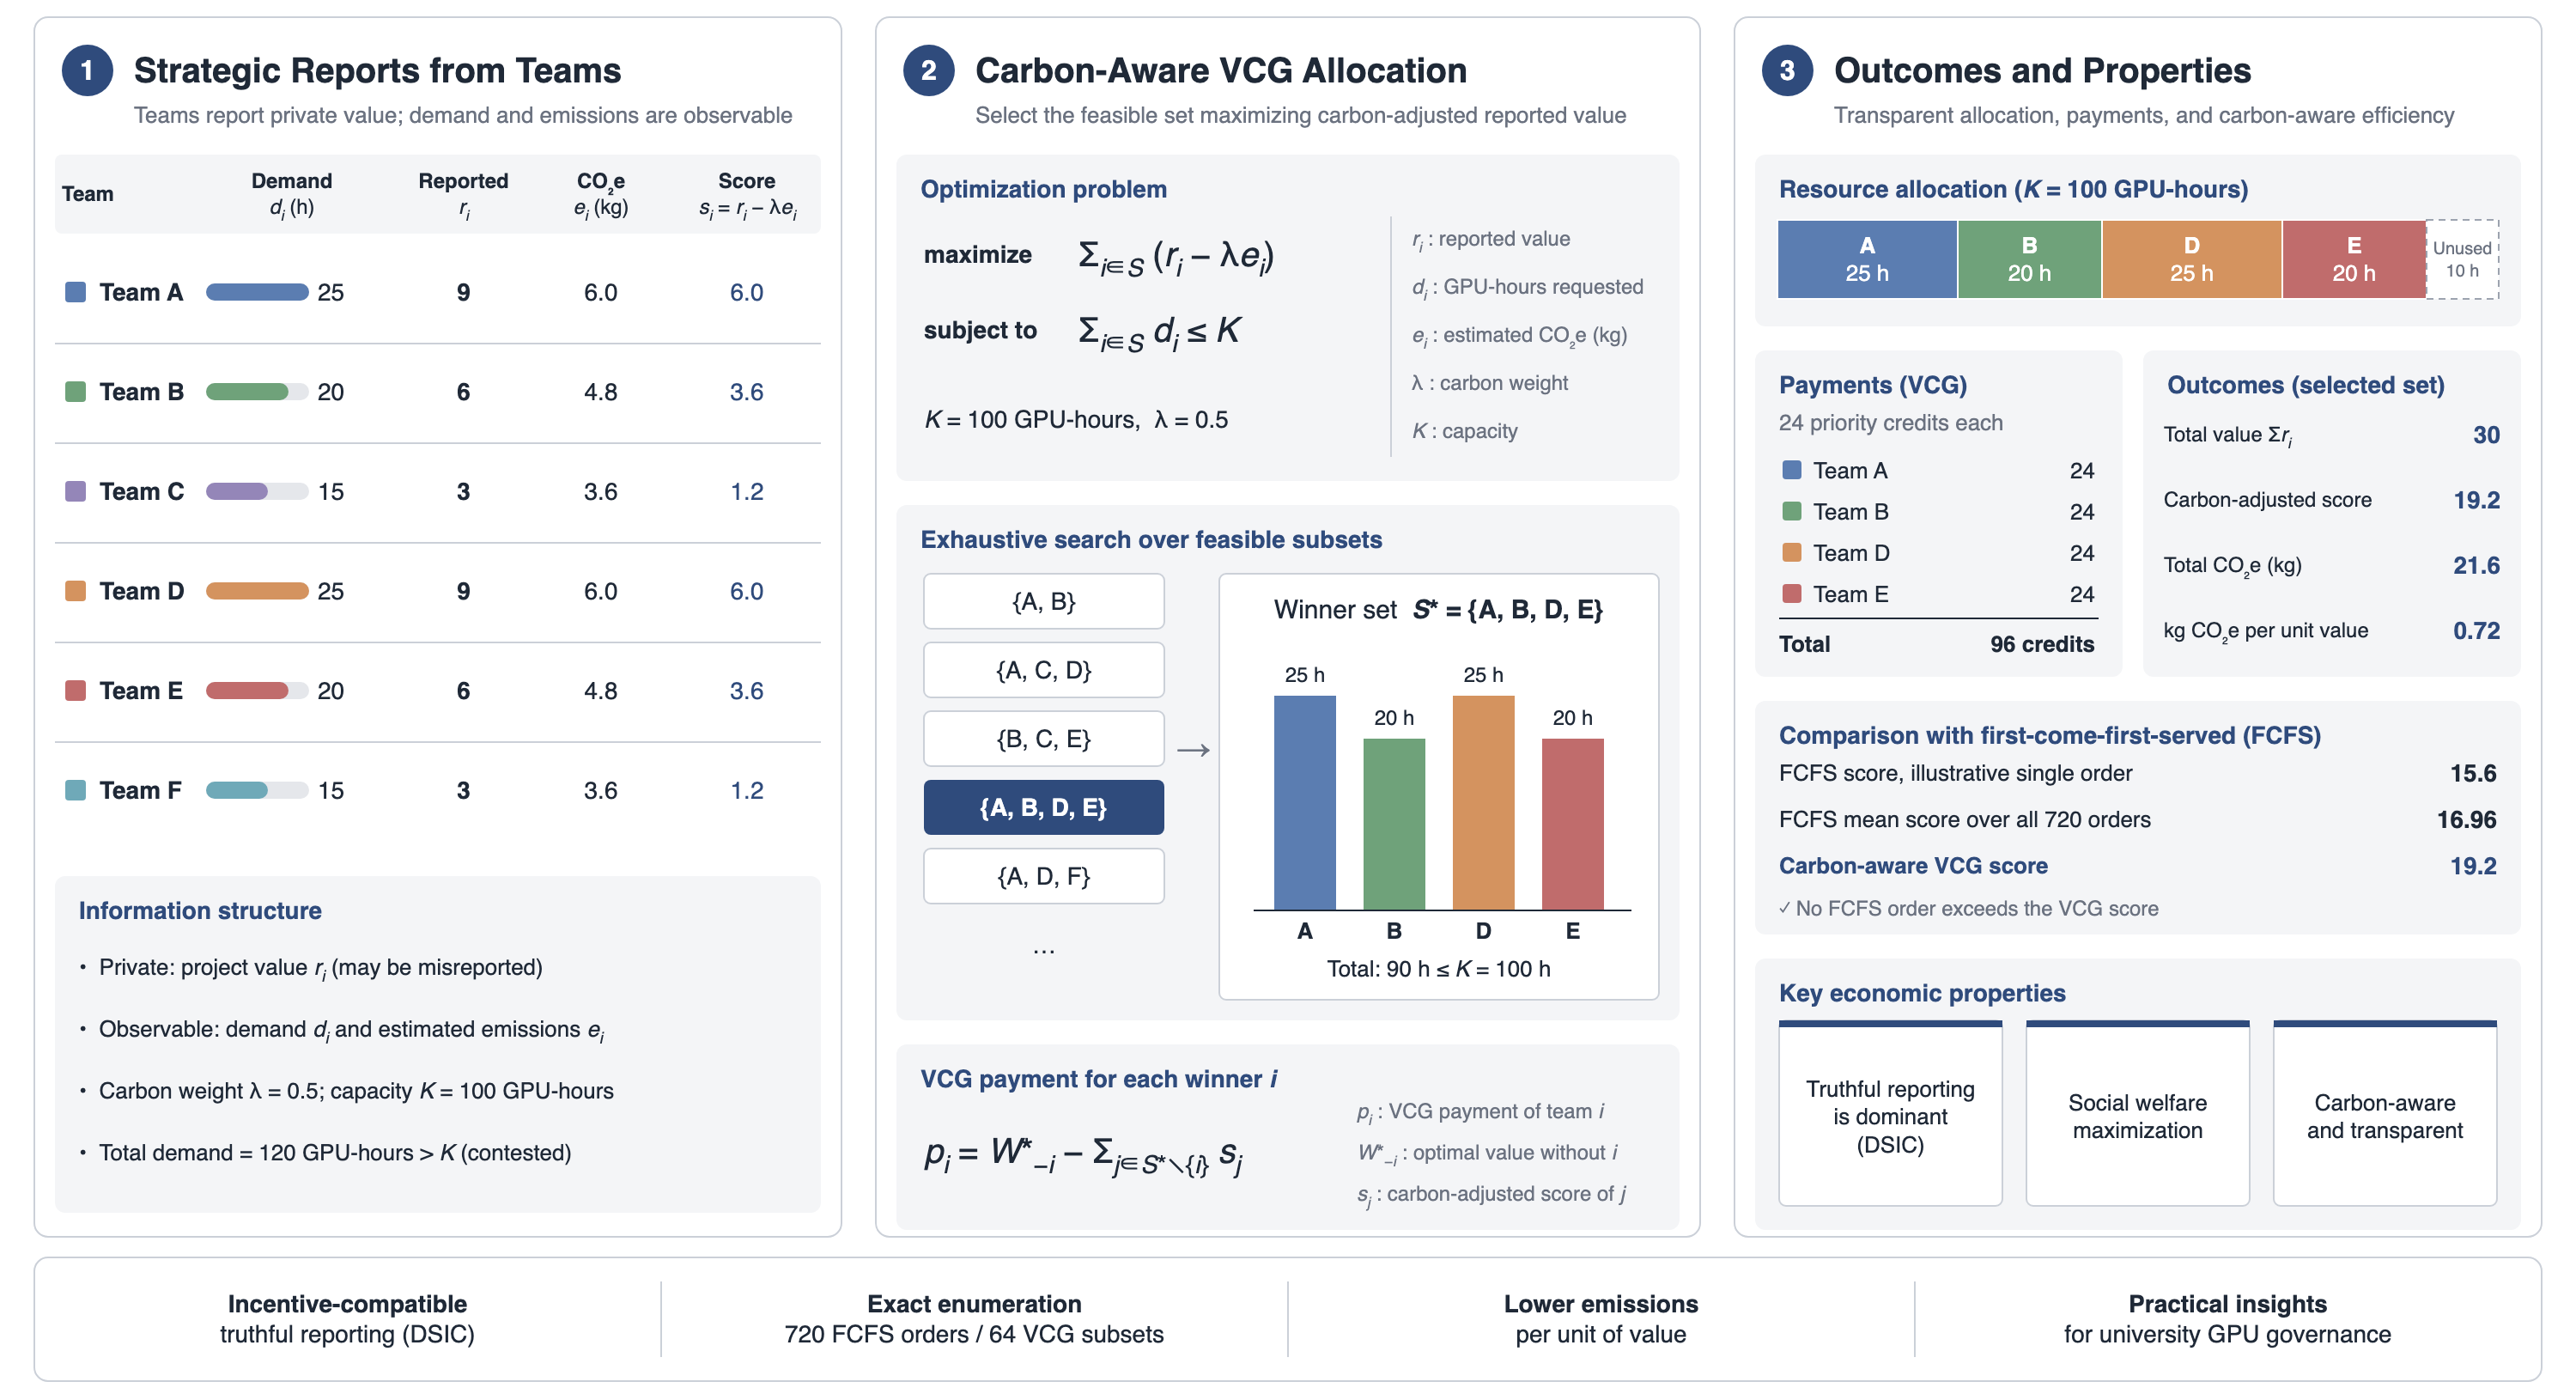
\includegraphics[
  width=\textwidth,
  keepaspectratio
]{figures/teaser_figure.png}
\caption{One integrated PS2 evidence chain. Economic reasoning defines the strategic question and institutional objective; reproducible computation tests the model; behavioral evidence probes assumptions; the A0 poster communicates the combined claim and its practical implications for a concrete real-world case. Replace every placeholder and distinguish completed evidence from planned work.}
\Description{Three disciplinary panels for economics, computer science, and behavioral science flow into an interdisciplinary synthesis bar linking the strategic claim, GitHub evidence, Hugging Face evidence, A0 poster, and real-world impact.}
\label{fig:teaser}
\end{teaserfigure}
\maketitle\raggedbottom\coursemeta

\noindent\textcolor{CourseTeal}{\textbf{PS1-continuous template.}} This file intentionally retains the PS1 ACM layout, five-section main paper, Author Notes, references, and Appendices A--E. Appendix F contains only the additional PS2 team, auction, linked-artifact, poster, and symposium records. Keep Sections 1--5 within two main pages, including metadata, Figure~\ref{fig:teaser}, its caption, and artifact links.

\section{Three connected research questions and verified gap}

\noindent
Universities increasingly compete for scarce GPU capacity as AI research outpaces compute budgets. First-come-first-served allocation ignores project value and urgency, wasting scientific value and unpriced carbon.

\vspace{3pt}

\noindent
The closest work, Zachariadis et al.'s FAIR-Compute report~\cite{fair_compute2026}, shows value-blind scheduling wastes a third of scientific value, but leaves incentive-compatible, carbon-aware allocation as unbuilt future work. We build exactly that, at small, exactly-solvable scale.

\vspace{3pt}

\noindent
\textbf{Q1---Economics:} How should an institution allocate scarce GPU-hours to maximize project value net of carbon cost, when teams privately know their own value and can misreport it?\par
\textbf{Q2---Computation:} Can an exactly-solvable multi-team VCG mechanism allocate more efficiently than first-come-first-served, while staying auditable?\par
\textbf{Q3---Behavior:} Do participants report values close to the truthful benchmark, or does behavior deviate---and do their predictions and reflections show understanding of the rule?

\vspace{3pt}

\noindent
Together: can a transparent, carbon-aware rule replace arrival order, and does its advantage survive behavioral and computational limits? Figure~\ref{fig:teaser} traces model (Q1) and its exact computation (Q2); the behavioral test (Q3) is described in Section 4.

\section{Answer to Q1: incentives and strategic model}

\noindent
\textbf{Hypothesis.} An incentive-compatible, carbon-aware mechanism increases realized value and reduces emissions per unit of value, without misreporting.

\vspace{3pt}

\noindent
\textbf{Model.} Six teams $i\in\{A,\dots,F\}$ compete for $K=100$ GPU-hours. Each privately knows value $v_i \in \{3,6,9\}$; demand $d_i$ is observable, emissions $e_i=0.24d_i$ kg CO$_2$e, carbon weight $\lambda=0.5$ (stated parameters, not empirical estimates). Teams simultaneously submit one report $r_i$ (static, incomplete information).

\vspace{3pt}

\noindent
\textbf{Allocation and payment.} Score $s_i=r_i-\lambda e_i$; select feasible $S^*$ maximizing $\sum_{i\in S}s_i$ s.t. $\sum_{i\in S}d_i\le K$ (demand enters only as the constraint). Each winner pays the Clarke--Groves externality $p_i = W_{-i}^* - \sum_{j\in S^*\setminus\{i\}}s_j$~\cite{clarke1971,groves1973} (Appendix~A); utility is $u_i=v_i-\lambda e_i-p_i$ if selected, else 0.

\vspace{3pt}

\noindent
\textbf{Solution concept.} Truthful reporting $r_i=v_i$ is dominant---stronger than Nash/Bayesian Nash equilibrium~\cite{nash1950,harsanyi1968}---holding only because each team bears its own carbon penalty in $u_i$ (else the optimum shifts to $r_i=v_i+\lambda e_i$) and credits carry real future cost; verified numerically over $[0,10]$ (Appendix~A.2).

\vspace{3pt}

\noindent
\textbf{Three lenses.} Game theory yields the dominant-strategy prediction; social choice frames value-net-of-carbon under capacity, surfacing an efficiency--access trade-off (Appendix~C); mechanism design specifies the report space, rules, and two verified tests (Appendix~C).

\section{Answer to Q2: computation, auction comparison, and artifacts}

\noindent
\textbf{Inputs.} Six teams (A--F): demands $(25,20,15,25,20,15)$, values $(9,6,3,9,6,3)$. FCFS is evaluated over all 720 arrival orders; VCG enumerates all 64 feasible subsets and re-solves per winner for payments (Appendix~A.1--A.2).

\textbf{Result.} VCG selects $\{A,B,D,E\}$ (score 19.2)---no FCFS order of 720 exceeds it (range 15.6–19.2; mean 16.96). Emissions per value fall from 0.81--0.84 to 0.72 kg CO$_2$e. One verified synthetic instance, not general evidence (Appendix~A, GitHub).

\section{Answer to Q3: behavior and interdisciplinary integration}

\noindent
\textbf{Rational benchmark.} Section~2 establishes $r_i=v_i$ as dominant under VCG; FCFS has no reporting decision at all.

\vspace{3pt}

\noindent
\textbf{Behavioral evidence.} Users experience FCFS, then report a value under VCG and predict their own selection---testing whether they report truthfully and understand the rule. Responses are exploratory only, not general behavioral evidence.

\vspace{3pt}

\noindent
\textbf{Interaction.} Users play one team through both FCFS and VCG stages, predicting their own selection before seeing the result, then inspect the ranking, payments, and utility (full mechanics in Appendix~F.1). All evidence is exploratory, with participant count and conditions reported.

\vspace{3pt}

\noindent
\textbf{Discriminating observation.} Misreporting with a wrong prediction suggests misunderstanding; misreporting with a correct prediction and a strategic reflection suggests genuine deviation---guiding interface or model revision, not causal claims.

\section{Advanced development, real-world impact, and roadmap}

\noindent
This proposal builds on two Nobel-recognized foundations: Vickrey's theory of incentives under asymmetric information~\cite{vickrey1961,nobel1996} and Hurwicz--Maskin--Myerson's mechanism design theory~\cite{nobel2007}---agents can be motivated to reveal the truth without verifying private information. GPU demand and carbon data are now specific enough to deploy this cheaply; only integrating both, plus a planned behavioral test, closes the two gaps left by Section~1's closest prior work.

\vspace{3pt}

\noindent
The concrete case is a shared university GPU cluster. Teams benefit from allocation reflecting true value; administrators gain an auditable record; the public bears the carbon cost regardless of who benefits. Honest reporting is incentivized, but truthfulness relative to a team's actual beliefs is not independently verifiable. Academic adoption would accept a transparent pilot; industry would demand robustness at hundreds of teams; public institutions would require an independently re-runnable audit. Next test: a pilot comparing self-reported value against ex-post outcomes at a scale where exact solving is no longer tractable.

\vspace{3pt}

\begin{table}[h]
\caption{From foundations to a collaborative interdisciplinary contribution.}
\begin{tabularx}{\columnwidth}{@{}p{1.6cm}Y@{}}
\toprule
\textbf{Horizon}&\textbf{Milestone and evidence}\\
\midrule
Foundation&Vickrey~\cite{nobel1996} and Hurwicz--Maskin--Myerson~\cite{nobel2007}: incentive-compatible allocation without verifying private information.\\
PS2&Six-team carbon-aware VCG mechanism, exactly solved and verified against a random-order first-come-first-served baseline over all 720 arrival orders (Appendix~A).\\
Symposium&Poster claim on institutional GPU governance; peer challenge on carbon-weight calibration and private-value verifiability; response via the audit-trail transparency argument.\\
Next study&Pilot comparing self-reported value against independent, ex-post project outcomes at a scale where exact solving is no longer tractable.\\
2056&Auditable mechanism-design tool adopted by a real institution for actual, not simulated, compute governance.\\
\bottomrule
\end{tabularx}
\end{table}

\vspace{3pt}

\noindent
\noindent\textbf{Expected 2056 Nobel Prize and Turing Award contribution statement.}
By 2056, we aim to be recognized for an efficient, publicly auditable governance framework for scarce shared infrastructure, integrating an incentive-compatible mechanism, verifiable computation, and behavioral evidence on truthful reporting. Progress moves from this six-team simulation to a real institutional pilot, correctable through a public, re-runnable audit log.

\subsection*{Open Science Statement}
GitHub (\url{https://github.com/GihoonE/COMPSCI206-PS2}) contains the FCFS/VCG code, tests, and outputs; a self-contained Colab notebook (\url{https://colab.research.google.com/drive/1uBTife193s0VDvmCZH3UQG1Q-UMNEcNx#scrollTo=f8338dd7}); a Hugging Face Space (\url{https://huggingface.co/spaces/dku-comsci-econ206-2026/PS2_Team_A}); README with run instructions. Inputs are synthetic ($d_i\in\{15,20,25\}$, $v_i\in\{3,6,9\}$; the Space allows continuous ranges), clearly labeled. Results from commit d93fc2e (tag ps2-review). Limitation: exact enumeration does not scale past small team counts.

\subsection*{Statement of Contribution to the UN's SDGs}
Connects to SDG~13 (carbon priced into allocation) and SDG~9 (auditable infrastructure rule). Audience: compute administrators and research teams; minimal access needs. Indicator: emissions per unit of allocated value. Possible unintended effect: urgency inflation beyond the report's resolution, or $\lambda$ disadvantaging compute-heavy research. Intended mechanism only---no adoption has occurred.
\clearpage\nobalance
\section*{Author Notes}
\subsection*{Acknowledgements}
\textbf{Course instructor: Professor Luyao Zhang.} We acknowledge the software this work relies on: Python and its standard library, Jupyter and Google Colab, matplotlib, and Hugging Face Spaces. Generative AI assistance is disclosed in Appendix~A.3. The authors remain responsible for the proposal and remaining errors.

\subsection*{Team and individual contributions}

\textbf{Joint contribution.} Our team studies how an organization can allocate scarce shared GPU-hours when teams privately know their project value but GPU demand and estimated emissions are observable. We compare a random-order FCFS baseline, computed over all 720 arrival orders, with a transparent carbon-aware VCG mechanism that selects a feasible group of teams under a 100 GPU-hour capacity limit. Temur supplies the formal model, exact computation, and reproducibility checks; Mustafa develops the social-choice, governance, and real-world-impact argument; Gihun develops the interactive explanation, artifact interface, and poster layout. These parts form one research argument: a stated allocation rule is useful only when its strategic assumptions, computational results, public explanation, and limits can be inspected together. All three members will jointly review the final paper and artifacts for consistency.

\textbf{Temur Akhtamjonov.} I designed the six-team GPU-allocation model, implemented the FCFS baseline and the exhaustive VCG solver, and verified the reported allocation, capacity, score, emissions, and payment outputs. My key decision was to model the setting as a multi-winner direct mechanism rather than a one-winner auction. My evidence is the GitHub simulation, runnable Colab notebook, and saved output files. This work provides the formal and computational basis for the paper, Hugging Face interaction, and poster. My next responsibility is to check that all three artifacts use the same parameters, allocation rule, and reported results.

\textbf{Mustafa Ayub Khan.} I developed the social-choice and mechanism-design framing: writing the literature review identifying FAIR-Compute as the closest prior work and the specific gap it leaves open---an incentive-compatible, carbon-aware allocation rule it names as future work but does not build---and drafting the real-world-impact case distinguishing academic, industry, and public-institution evidence standards for adoption. My key decision was identifying that an early fixed-price allocation formula (score proportional to GPU-hours alone) had silently dropped private project value from the mechanism, and proposing the corrected selection rule $s_i = r_i - \lambda e_i$, which restores private value as the basis for selection and keeps demand as only a capacity constraint---the formula the team's VCG mechanism is built on. I also treated auditability of execution, not verification of private values, as the honest limit of this mechanism's transparency. My evidence is Sections~1, 2, and~5, the Open Science and SDG statements, and Table~1's roadmap. I independently re-derived Temur's FCFS and VCG allocation numbers by hand against the stated $v_i$, $d_i$, and $\lambda=0.5$, confirming the reported subsets, scores, and total payment of 9.6 score units (96 priority credits). This argument depends on Temur's simulation producing the value/carbon trade-off Section~5 describes, and feeds the poster's real-world-case panel and Gihun's audit-trail framing in the Hugging Face interface. My next responsibility is to check symposium feedback against Section~5's adoption-evidence claims and revise the real-world case accordingly.

\textbf{Gihun Lee.} I built the public-facing allocation audit and the reproducibility interface: the Hugging Face Space, the GitHub README, the self-contained Colab notebook structure, Figure~\ref{fig:teaser}, and the poster layout. My key decision was to make the stated rule checkable against its visible execution: in the Space a player holds a private true value, reports separately, predicts their own selection, and then sees the score ranking, winning group, VCG payments, utility, and a what-if curve of utility against every report. While building this audit, I found that the original utility $v_i-p_i$ contradicted the paper's dominant-strategy claim, because under it a team gains by reporting $v_i+\lambda e_i$. I proposed $u_i=v_i-\lambda e_i-p_i$, added a truthfulness sweep, and replaced the single FCFS queue with all 720 arrival orders. My evidence is the Space, the \texttt{colab/} folder (tests, outputs, notebook), and the README. I verified that the unit tests pass, that the notebook runs 7/7 checks in a clean folder without the repository, that the browser port matches the Python code on 300 random games, and that \texttt{run\_simulation.py} reproduces the committed outputs. This work turns Temur's computation and Mustafa's framing into an interface a non-specialist can inspect. My next responsibility is to run classroom peer-play at the symposium, report the number of participants as exploratory evidence, and keep the poster, paper, and artifacts at parity through the September 30 revision.

\bibliographystyle{ACM-Reference-Format}\bibliography{references}
\appendix
\section{Technical details and reproducibility}

\subsection{Model inputs and rules}

This project uses one fixed synthetic classroom example with six teams and a capacity of $K=100$ GPU-hours. Table~\ref{tab:inputs} gives the inputs. Values are private to teams but are reported truthfully in the baseline computation. GPU-hour demand is observable. Estimated emissions use the stated classroom assumption $e_i=0.24d_i$ kg CO$_2$e. The announced carbon weight is $\lambda=0.5$, so each reported score is
\[
s_i=r_i-\lambda e_i=r_i-0.5(0.24d_i).
\]

\begin{table}[h]
\centering
\caption{Fixed synthetic inputs used in the fresh run.}
\label{tab:inputs}
\begin{tabular}{lrrr}
\toprule
Team & GPU-hours $d_i$ & Value $v_i$ & Emissions $e_i$ \\
\midrule
A & 25 & 9 & 6.0 \\
B & 20 & 6 & 4.8 \\
C & 15 & 3 & 3.6 \\
D & 25 & 9 & 6.0 \\
E & 20 & 6 & 4.8 \\
F & 15 & 3 & 3.6 \\
\bottomrule
\end{tabular}
\end{table}

The FCFS baseline uses a random arrival order. Each team receives its full request only when the request fits in the remaining capacity. We compute all $6!=720$ orders exactly and report A, B, E, C, D, F as one illustrative draw. The proposed mechanism is a simultaneous-report, multi-winner VCG direct mechanism. It chooses the feasible subset $S$ that maximizes total reported score:
\[
\max_{S \subseteq N}\sum_{i\in S}s_i
\quad \text{subject to} \quad
\sum_{i\in S}d_i\leq K.
\]
For each selected team $i$, the priority-credit payment is its reported-score externality:
\[
p_i=
\max_{S'\subseteq N\setminus\{i\}}\sum_{j\in S'}s_j
-
\sum_{j\in S\setminus\{i\}}s_j.
\]
One payment score unit equals 10 non-transferable priority credits in this classroom model. A selected team's utility is $u_i=v_i-\lambda e_i-p_i$, and an unselected team's utility is $0$. Each team bears its own carbon penalty; this is what makes truthful reporting dominant.

\subsection{Exact algorithm and fresh-run record}

The implementation checks every possible subset of six teams.

\begin{enumerate}
\item Enumerate all $2^6=64$ subsets.
\item Remove a subset if its total requested GPU-hours exceed 100.
\item Compute total reported score for every remaining subset.
\item Select the subset with the largest score. Ties are broken publicly by first serving more teams and then using deterministic team order.
\item For each selected team, repeat the calculation without that team and compute its externality payment.
\item Truthfulness check: for each team, re-run steps 1--5 with its report set to $0,0.5,\dots,10$, holding the other teams fixed, and confirm that no report beats $r_i=v_i$.
\end{enumerate}

A fresh run of \texttt{python colab/run\_simulation.py} reproduces the saved summary, team-level, all-orders, and truthfulness CSV outputs in the repository's \texttt{colab/outputs} folder. The same calculation is available in our self-contained Colab notebook (\NotebookLink).

The saved fresh-run comparison is:

\begin{center}
\small\setlength{\tabcolsep}{3pt}
\begin{tabularx}{\columnwidth}{@{}Yrrrr@{}}
\toprule
Rule & GPU-h & Value & CO$_2$e & Score \\
\midrule
FCFS (A,B,E,C,D,F) & 95 & 27 & 22.8 & 15.6 \\
FCFS, 720-order mean & 97.0 & 28.6 & 23.28 & 16.96 \\
VCG (A,B,D,E) & 90 & 30 & 21.6 & 19.2 \\
\bottomrule
\end{tabularx}
\end{center}

In the illustrative order, FCFS serves A, B, E, C, and F and leaves 5 GPU-hours unused. Across all 720 orders, the FCFS carbon-adjusted score ranges from 15.6 to 19.2, and no order exceeds VCG. VCG leaves 10 GPU-hours unused and collects 9.6 payment score units, equal to 96 priority credits (2.4 per winner). Utilities are 3.6 for A and D, 1.2 for B and E, and 0 for C and F. For every team, no report in $[0,10]$ yields higher utility than $r_i=v_i$. The notebook's final cell prints PASS for seven checks: allocation, capacity, value and score, payments, utilities, truthful optimality, and the 720-order comparison. A repository test confirms that the notebook's model code is identical to \texttt{colab/src/gpu\_allocation.py}.

\subsection{Reproducibility, limits, and AI-use disclosure}

\textbf{Reproducibility.} The GitHub repository (\GitHubLink) contains the source code, tests, notebook, output files, and README instructions in \texttt{colab/}. The model, script, and tests use only the Python standard library. The notebook's utility plot uses matplotlib, which Colab provides. Reported results come from commit \texttt{d93fc2e}.

\textbf{Limits.} This is a small synthetic example, not a field deployment. The 0.24 kg CO$_2$e per GPU-hour rate, the carbon weight, the value tiers, and the 10-credit conversion are classroom assumptions. Exact enumeration will not remain practical as the number of teams becomes large. The model also cannot verify a team's true private value.

\textbf{AI-use disclosure.} The team used Claude Code (Claude Opus 5.5, Anthropic) on September 25--26, 2026. It was used to build the Hugging Face Space, restructure the README, self-contained notebook, write the simulation codes and unit tests, and draw Figure~\ref{fig:teaser}. 

\section{Cumulative Intellectual Development}
\textbf{Mustafa Ayub Khan -- prior development.} In PS1, Mustafa studied whether greater observability changes voluntary disclosure in a public-goods setting. Following Professor Zhang's September 7 feedback, he narrowed the claim and proposed a 2-by-2 design to distinguish genuine behavioral change from merely visible performance. This led to one bounded lesson for PS2: making a rule and its execution observable can improve accountability, but it cannot prove that a participant's private motive or value report is true. In the GPU-allocation project, this lesson appears in the published allocation rule, parameters, code, payments, and allocation log.

\textbf{Gihun Lee -- prior development.} In PS1, Gihun developed a transparent way to compare heterogeneous AI subscription plans using workload-specific measures, reproducible computation, sensitivity checks, and a public-facing interaction. Feedback on trustworthiness led him to avoid one opaque summary number and instead show the underlying components and assumptions. In PS2, this becomes the Hugging Face allocation audit: users can compare FCFS and the VCG mechanism, inspect the reported inputs and outcomes, see the stated assumptions behind the result, and check with a what-if curve whether truthful reporting maximizes their own utility.

\textbf{Temur Akhtamjonov -- development into the shared model.} Temur's earlier work on a commitment-bond trust game used a clear benchmark, a controlled rule change, and verified computational outputs. In PS2, he transfers this methodological approach to a new shared setting: hold the six-team GPU environment fixed, compare FCFS with carbon-aware VCG, enumerate all feasible allocations exactly, and report the resulting allocation and payments.

\textbf{Intellectual consequence.} PS2 is a new joint project, not a continuation of one PS1 topic. Its common development is methodological: each prior project emphasized a clear rule, visible assumptions, reproducible computation, and careful limits on what observed behavior can establish. Our shared contribution applies these principles to a transparent, carbon-aware allocation of scarce organizational GPU-hours.

\section{Open-source and three-lens inspiration}
\textbf{Sources and tools.} PS1 source records are preserved in each author's PS1 submission; the tools below are those used in PS2.

{\footnotesize
\begin{tabularx}{\columnwidth}{@{}p{1.6cm}Y@{}}\toprule
\textbf{Source / tool}&\textbf{URL, license, version; capability; limitation; design consequence}\\\midrule
Python standard library&\url{https://www.python.org}; PSF License; 3.13--3.14 locally, Colab runtime. Exact subset enumeration and permutations with no installs. Exponential in team count. Kept the model dependency-free so anyone can re-run it.\\
Jupyter / Google Colab&\url{https://jupyter.org} (BSD-3), \url{https://colab.research.google.com} (Google service terms). Runnable notebook with saved outputs. Hosted runtime can change over time. Notebook made self-contained, with a test that it matches \texttt{src/}.\\
matplotlib&\url{https://matplotlib.org}; matplotlib license (PSF-based); 3.11. Utility-versus-report plots. Plots only. Used only outside the model code.\\
Hugging Face Spaces (static)&\url{https://huggingface.co/docs/hub/spaces-sdks-static}; hosted service. Serves an HTML/CSS/JS page with no server. Cannot store responses. Evidence is collected by participants copying a result line rather than by server logging.\\
Claude Code&\url{https://claude.com/claude-code}; Anthropic terms; Claude Opus 5.5, Sept.~2026. Coding and drafting assistant. Can err, so all outputs were tested. See Appendix~A.3.\\\bottomrule
\end{tabularx}}

\textbf{How each lens altered the shared model.}
\emph{Game theory:} framing the setting as a static game with incomplete information made $r_i=v_i$ the benchmark to test. Testing it (observation) showed that the original utility $v_i-p_i$ rewards overreporting by $\lambda e_i$, so the utility now includes each team's own carbon penalty.
\emph{Social choice:} stating the objective as value net of carbon under capacity exposed the efficiency--access trade-off. VCG serves 4 teams against an FCFS mean of 4.93 (observation). We interpret this as a real cost of the rule rather than a flaw to hide.
\emph{Mechanism design:} it fixed the report space, allocation, payment, and public tie-break, and it turned FCFS from one arbitrary queue into all 720 orders. The $\lambda$ sensitivity (observation) shows that the carbon weight changes the winning group between $\lambda=0$ and $\lambda=0.5$.
All three results are computed from the formal model. Whether people report truthfully is planned classroom evidence, not yet observed.

\section{Review response and revision record}
\textbf{Status.} This is the review-ready version (v1). Peer reviews (two per student), discussant comments, and instructor feedback will be collected at the symposium on Monday, September 28, 2026, and recorded here with Keep, Revise, or Investigate decisions, changed locations, and rerun results in the final version (v2, September 30, 2026).

\clearpage\onecolumn
\section{Structured abstract and cumulative proposal map}\label{app:abstract}
PS2 is a new topic; the PS1 map is preserved in each author's PS1 submission. The table below is the PS2 review-ready version (v1).
\par\medskip
\begin{table}[H]
\caption{Structured abstract and cumulative proposal map (PS2, review-ready v1).}
\label{tab:abstract-map}
\renewcommand{\arraystretch}{1.18}
\begin{tabularx}{\textwidth}{@{}p{0.27\textwidth}Y@{}}
\toprule
\textbf{Proposal element} & \textbf{Current statement / change} \\
\midrule
Background & Setting: several teams compete for scarce shared GPU-hours; each knows its own project value, while requests and emissions are public. Established: VCG mechanisms (Vickrey; Clarke; Groves) allocate efficiently with truthful reporting as a dominant strategy. Unresolved: institutional GPU allocation is often queue-based, blind to both value and carbon. Foundation: Vickrey (1996 Nobel) and Hurwicz--Maskin--Myerson (2007 Nobel). \\
Motivation and application & AI research demand outpaces compute budgets now. Case: a university's shared GPU cluster with 100 GPU-hours and six project teams. Affected: research teams (who gets compute), administrators (who must justify allocations), and the public (carbon cost). Need: a rule that is efficient, carbon-aware, and auditable. \\
Three connected questions & Economics: how to allocate GPU-hours to maximize value net of carbon when values are private and can be misreported? Computation: can an exactly solved multi-team VCG outperform FCFS while staying auditable? Behavior: do participants report truthfully and understand the rule? Integrated: can a transparent, carbon-aware rule replace arrival order, and does its advantage survive behavioral and computational limits? \\
Method and model assumptions & Actors: six synthetic teams A--F. Information: private $v_i\in\{3,6,9\}$; public $d_i$ and $e_i=0.24d_i$; $\lambda=0.5$. Timing: one simultaneous report $r_i$. Model: static game with incomplete information; solution concept DSIC, with $u_i=v_i-\lambda e_i-p_i$. Baseline: random-order FCFS over all 720 orders. Computation: exact 64-subset VCG and a truthfulness sweep (GitHub, Colab). Evidence: Hugging Face play. \\
Results or expected results & Actual (computed, synthetic): VCG selects A, B, D, E, using 90 GPU-hours, value 30, score 19.2, 21.6 kg CO$_2$e, and 96 credits. FCFS scores 15.6 in the illustrative order and 16.96 on average over 720 orders, and no order beats VCG. Truthful reporting is optimal for every team. Planned (behavioral): classroom play recording reports, predictions, and reflections. Falsifier: users who predict the outcome correctly but still misreport; or, computationally, any misreport or FCFS order that beats the reported benchmark. \\
Intellectual merits & Integrating a carbon objective with incentive compatibility changes the design: truthful reporting holds only if each team bears its own carbon penalty in its utility. An exact, small-scale audit makes every allocation, payment, and utility re-checkable by a reader. \\
Practical impacts & Private value: teams get compute by value, not arrival order. Public value: lower emissions per unit of value (0.72 vs.\ 0.81--0.84 kg). Access: VCG serves fewer teams (4 vs.\ 4.93). Risks: $\lambda$ may disadvantage compute-heavy research; values cannot be verified; credits need real future cost. Evidence needed: a pilot comparing reported value with ex-post outcomes. Correction: a public, re-runnable audit log. SDG 13 (carbon priced into allocation) and SDG 9 (auditable infrastructure rule). \\
Feedback received and revision made & (1) Internal audit, Sept.~25--26, 2026 (Gihun): earlier claim was DSIC under $u_i=v_i-p_i$. Decision: Revise. The utility now includes the own carbon penalty, and a truthfulness sweep was added. Verified by unit tests and a notebook fresh run. Consequence: winners' utilities changed (A and D from 6.6 to 3.6). (2) Mustafa's model review: an earlier score used GPU-hours alone. Decision: Revise to $s_i=r_i-\lambda e_i$. (3) FCFS generality: Revise from one fixed queue to all 720 orders. Peer and instructor feedback from September 28 will be added in v2. \\
\bottomrule
\end{tabularx}
\end{table}
\noindent Keep detailed technical records, literature notes, open-source inspirations, acknowledgements, and AI-use disclosure in the supporting sections. The main paper, linked artifacts, poster, and structured abstract must use the same question, assumptions, and evidence status.
\clearpage\twocolumn
\section{PS2 extension record: auction, linked artifacts, poster, and symposium}
\subsection{Auction laboratory record}

\textbf{Rules (all treatments).} Resource: $K=100$ GPU-hours; six teams A--F with demands $(25,20,15,25,20,15)$ and true values $(9,6,3,9,6,3)$; $e_i=0.24d_i$, $\lambda=0.5$.
\emph{FCFS:} teams arrive in a random order; each full request is granted if it fits in the remaining capacity, otherwise skipped; no payment; the rule stops after the last arrival.
\emph{Carbon-aware VCG:} one sealed, simultaneous report $r_i$ per team; the rule selects the feasible group $S^*$ maximizing $\sum_{i\in S}(r_i-\lambda e_i)$ (ties: more teams, then earlier team); each winner pays $p_i=W^*_{-i}-\sum_{j\in S^*\setminus\{i\}}(r_j-\lambda e_j)$ score units ($\times10$ priority credits); the rule stops after this single round.
Utility: $u_i=v_i-\lambda e_i-p_i$ if selected, else $0$. Efficiency: realized carbon-adjusted \emph{true} score divided by the optimum, 19.2.

{\footnotesize
\begin{tabularx}{\columnwidth}{@{}p{1.45cm}YYY@{}}\toprule
 & \textbf{T1 FCFS} & \textbf{T2 VCG, truthful} & \textbf{T3 VCG, C overreports}\\\midrule
Identifier & \texttt{fcfs\_allocation}, \texttt{fcfs\_all\_orders} & \texttt{vcg\_allocation} & \texttt{misreport\_sweep} (team C)\\
Settings & 720 orders; shown: A,B,E,C,D,F & baseline & C reports 4.5; others truthful\\
Value & $v=(9,6,3,9,6,3)$ & same & same; $v_C=3$\\
Planned bid & none (request $d_i$ only) & $r_i=v_i$ & $r_C=4.5$\\
Prediction & no report incentive & truthful is dominant (DSIC) & C's utility falls\\
Outcome & A,B,E,C,F; 95\,h & A,B,D,E; 90\,h & A,B,C,D,F; 100\,h\\
Payment & 0 & 2.4 each (24 cr.) & A,B,D 3.6; C 2.4; F 0.9\\
Utility & A 6, B 3.6, E 3.6, C 1.2, F 1.2, D 0 & A,D 3.6; B,E 1.2; C,F 0 & C $-1.2$ (vs.\ 0 truthful)\\
Revenue & 0 & 9.6 (96 cr.) & 14.1 (141 cr.)\\
Efficiency & 81.3\% (shown order); mean 88.3\% over 720 & 100\% & 93.8\% (score 18.0)\\
Emissions & 22.8 (mean 23.28) kg & 21.6 kg & 24.0 kg\\
Behavior & none: computed & none: computed & none: computed\\
Revision & single order $\to$ all 720 orders & utility now includes own $\lambda e_i$ & confirms truth is optimal for all teams\\\bottomrule
\end{tabularx}}

\textbf{Hugging Face play.} A participant plays one team with a private true value $v_i\in\{1,\dots,10\}$ and a request $d_i\le30$; five rivals are simulated and truthful. Stage~1 is FCFS; in Stage~2 the participant reports $r_i$, predicts whether the team is selected, then sees the ranking, winning group, payments, utility, and a what-if curve of $u_i(r_i)$. Recorded per play (copied by the participant): $d_i$, $v_i$, $r_i$, prediction, outcome, payment, utility, preferred rule, and reflection. No plays have been collected yet; any results will be reported as exploratory, with the number of participants.

\subsection{Linked-artifact parity}
{\footnotesize
\begin{tabularx}{\columnwidth}{@{}p{1.75cm}Y@{}}\toprule
\textbf{Artifact}&\textbf{Required parity check}\\\midrule
GitHub&Model: \texttt{colab/src/gpu\_allocation.py}. Inputs: $K=100$, $d=(25,20,15,25,20,15)$, $v=(9,6,3,9,6,3)$, $\lambda=0.5$, 0.24\,kg/GPU-h, 10 cr./unit. Commit \texttt{d93fc2e}. Runnable path: \texttt{python colab/run\_simulation.py}; tests: \texttt{cd colab \&\& python -m unittest discover -s tests}. Output: \texttt{colab/outputs/*.csv}; FCFS 15.6 vs.\ VCG 19.2, 96 credits. \\
Colab&\NotebookLink: self-contained copy of the same model code; a repository test checks that its model cells equal \texttt{src/}. Fresh-run cell: 7/7 checks PASS.\\
Hugging Face&Same decision setting (100 GPU-h, six teams, $e_i=0.24d_i$, $\lambda=0.5$, same FCFS and VCG rules, same tie-break, same utility). Browser port of the model, cross-checked against Python on 300 random games. Behavioral assumption: rivals truthful; benchmark $r_i=v_i$. Evidence status: observed (own choices), simulated (rivals), computed (outcomes), planned (classroom play). Privacy: nothing is stored or sent; players copy their own result line.\\
A0 poster&``Can a carbon-aware VCG rule allocate shared GPU-hours better than first come, first served?'' (A0 landscape, review-ready v1, Sep.~27). Same three-part structure (question \& model; design \& evidence; impact \& dialogue), inputs ($K=100$, six teams, $e_i=0.24d_i$, $\lambda=0.5$), payoff $u_i=v_i-\lambda e_i-p_i$, and results: VCG $\{A,B,D,E\}$, score 19.2 vs.\ FCFS mean 16.96; 0.72 vs.\ 0.81\,kg CO$_2$e per value; 4 vs.\ 4.93 teams served. Fig.~2 plots all 720 FCFS orders and Team C's misreport sweep. Real-world case, limitations, reviewer question, instructor, acknowledgements, and QR codes to the Space and GitHub (commit \texttt{d93fc2e}). Evidence status matches: computed; behavioral play planned.\\\bottomrule
\end{tabularx}}

\end{document}
